\documentclass[11pt,a4paper]{ltxdoc} 
\usepackage[spanish,es-noindentfirst,es-tabla]{babel}

\usepackage[utf8]{inputenc}
\usepackage[T1]{fontenc}
\usepackage{graphicx}
\usepackage{float}
\usepackage{xcolor}
\usepackage[margin=2.5cm,left=3.5cm]{geometry}

\setlength{\parskip}{0.2\baselineskip}
\renewcommand{\baselinestretch}{1.1}

\newcommand{\file}[1]{\texttt{#1}}
\newcommand{\option}[1]{\texttt{#1}}
\newcommand{\package}[1]{\texttt{#1}}

\title{\file{aleph-examen.cls}}
\author{Proyecto Alephsub0\\ Andr\'es Merino}
\date{2020-08-15\\ Versión 1.0}

\usepackage[colorlinks,linkcolor=teal,urlcolor=teal,
   citecolor=black,bookmarks=true]{hyperref}
\usepackage{url}

\begin{document}
 
\maketitle
 
\begin{abstract}
    \file{aleph-examen.cls} es una clase creada para dar formato a exámenes y hojas de ejercicios. Esta clase fue generada dentro del proyecto Alephsub0 (\url{https://www.alephsub0.org/}).
\end{abstract}

\section{Introducción}

La clase \file{aleph-examen.cls} es parte del conjunto de clases y paquetes creados por Andrés Merino. Esta clase provee el formato para generar exámenes, pruebas, hojas de ejercicios, hojas de datos y hojas de respuestas. En especial, las hojas de datos y de respuestas están enfocadas a la toma de pruebas masivas que tienen lugar en la Escuela Politécnica Nacional.

\section{Uso}

Para cargar la clase se utiliza: \cs{documentclass}\oarg{opciones}|{aleph-examen}| con las opciones acordes al formato que se desee.

Para visualizar un ejemplo puedes acceder al repositorio de GitHub de esta clase (clic \href{https://github.com/mate-andres/LaTeX_aleph-examen}{aquí}) o buscarlo en la galería de plantilla de Overleaf (clic \href{https://www.overleaf.com/latex/templates/plantilla-para-generar-examenes-de-ecfm/wcchsrcqqrxm}{aquí}).

\subsection{Opciones}

Las opciones de la clase son las siguientes:
\begin{description}
    \item[|10pt|, |11pt|, |12pt|] ajustan el tamaño de fuente.
    \item[|a4|, |a5|,|compacto|] genera la geometría de página y márgenes. Las dimensiones generadas por estas opciones están dadas en la Tabla~\ref{tab:01}.
    \item[|respuestas|] indica si se agregan o no las soluciones.
\end{description}
  
\begin{table}[ht]
    \centering
    \begin{tabular}{cccc}\hline
        Opción & Dimensiones & Laterales & Superior e Inferior \\\hline
        |compacto| & 160$\times$240 mm & 1.0 cm & 0.5 cm\\
        |a4| & A4 & 1.5 cm & 1.0 cm \\
        |a5| & A5 & 1.0 cm & 0.5 cm \\
        \hline
    \end{tabular}
    \caption{Geometría de página predefinida.}
    \label{tab:01}
\end{table}

\subsection{Colores}

Las clase trabaja con un color básico:
\begin{description}
    \item[|colortext|] es el color preestablecido para los enunciados bajo la opción |respuestas|. El color predefinido por la clase es |blue!50!black|.
\end{description}
Se puede cambiar fácilmente este color con los comandos\\
    \hspace*{3em}\cs{definecolor}|{colortext}|\marg{formato de color}\marg{color}\\
o\\
    \hspace*{3em}\cs{colorlet}|{colortext}|\marg{color}

\subsection{Comandos de datos del examen}

\DescribeMacro{\universidad} 
    El comando universidad tiene el formato\\
        \hspace*{3em}\cs{universidad}\marg{nombre de la universidad}.\\
    este comando es opcional, de no estar presente, el nombre de universidad por defecto es Escuela de Ciencias Físicas y Matemática (lugar donde trabaja actualmente el autor de la clase).

\DescribeMacro{\carrera} 
\DescribeMacro{\materia}
\DescribeMacro{\examen}
\DescribeMacro{\autor}
\DescribeMacro{\fecha} 
    Los comandos \cmd{\carrera} (opcional), \cmd{\materia}, \cmd{\examen}, \cmd{\autor} y \cmd{\fecha} dan la información que se utilizará en el encabezado, todas estas son obligatorias para generar exámenes u hojas de datos. No son empleadas al generar hojas de respuestas (no es necesarios incluirlos en estas hojas). El contenido de \cmd{\materia} y \cmd{\examen} se despliega en forma centrada mientras que el de \cmd{\autor} y \cmd{\fecha} se despliega en los extremos de la página.

\DescribeMacro{\hoja}
\DescribeMacro{\tema}
    Los comandos \cmd{\hoja} y \cmd{\tema} agregan información para el encabezado pero son opcionales. Se utiliza el comando \cmd{\hoja} para establecer si se trata de una hoja de enunciado o de datos.

\DescribeMacro{\notapie}
\DescribeMacro{\firma}
    Los comandos \cmd{\notapie} y \cmd{\firma} agregan información al final de la evaluación, luego de la linea final. Se utilizan para agregar notas al pie y firma de autoría.

\DescribeMacro{\logouno}
\DescribeMacro{\logodos}
    Los comandos \cmd{\logouno} y \cmd{\logodos} definen el archivo de logo a ser utilizado, ninguno de los dos es obligatorio. Cada comando tiene un argumento opcional en el cual se puede especificar el tamaño del logo.

\DescribeMacro{\Npreguntas}
    El comando \cmd{\Npreguntas} guarda la información del número de preguntas para generar el cuadro de información en la hoja de datos. No es necesario si no se utiliza el comando |\codigo|.


\subsection{Comandos}

\DescribeMacro{\encabezado}
    El comando \cmd{\encabezado} genera el encabezado de la página, no tiene ninguna opción.


\DescribeMacro{\EnExamen}
\DescribeMacro{\EnRespuesta}
    Los comandos \cmd{\EnExamen} y \cmd{\EnRespuesta} generan material que únicamente se desplegará si está habilitada o inhabilitada la opción |respuestas| en las opciones de la clase.

\DescribeMacro{\datosF}
\DescribeMacro{\datosN}
\DescribeMacro{\datosP}
    Los comandos \cmd{\datosF} y \cmd{\datosS} generan líneas para que el alumnos pueda colocar sus datos, tanto para datos de Formación Básica de la EPN (\cmd{\datosF}) como para datos de Nivelación de la EPN (\cmd{\datosN}) estas lineas solo se despliegan fuera de la opción |respuestas|. El comando \cmd{\datosP} genera líneas para los datos usuales solicitados en la PUCE.

\DescribeMacro{\opciones}
\DescribeMacro{\opcionesl}
    El comando \cmd{\opciones} tiene cuatro argumentos obligatorios y genera una lista de cuatro literales para las preguntas de opción múltiple, su sintaxis es:\\
        \hspace*{3em}\cs{opciones}\marg{Op1}\marg{Op2}\marg{Op3}\marg{Op4}.\\
    El comando \cmd{\opcionesl} es similar al anterior, pero despliega las opciones en una sola línea. 
    
\DescribeMacro{\puntaje}
    El comando \cmd{\puntaje} coloca el puntaje al final de cada pregunta.
    
\DescribeMacro{\codigo}
    El comando \cmd{\codigo} tiene cinco argumentos obligatorios y sirve para generar hojas de código de cada estudiante, su sintaxis es:\\
        \hspace*{3em}\cs{codigo}\marg{Nombre}\marg{Código}\marg{Grupo CD}\marg{Grupo CP}.

\DescribeMacro{\cuadro}
    El comando \cmd{\cuadro} genera un cuadro en blanco, útil para generar las hojas de respuestas. Este comando posee una opción la cual es el texto del cual se quiere medir el tamaño para generar el cuadro.

\DescribeMacro{\HojaRespuesta}
    El comando \cmd{\HojaRespuesta} genera la hoja de respuestas estandar, este comando posee una opción que se utiliza para colocar más información en esta hoja.
  
\subsection{Ambientes}

\DescribeEnv{preguntas}
    El ambiente |preguntas| genera una lista a la cual se le puede agregar cualquier opción del paquete |enumitem|.
    
\DescribeEnv{indicaciones}
    El ambiente |indicaciones| genera una lista en letra pequeña con el título de ``Indicaciones''. No confundir con el comando |\indicacionesHD|, no utilizar este ambiente al generar la hoja de datos.

\DescribeMacro{\indicacionesHD}
    El comando \cmd{\indicacionesHD} guarda la información de indicaciones para generar hojas de datos. Este comando es útil únicamente en las hojas de datos pues guarda las indicaciones para replicarlas en cada hoja. 
    
\DescribeEnv{respuesta}
    El ambiente |respuesta| genera un ambiente |proof| para la redacción de las respuestas a las preguntas. Las preguntas van tituladas por ``Solución'' de manera predefinida, esta se puede cambiar como una opción del paquete.
    
    El contenido del ambiente |respuesta| únicamente de desplegará cuando la opción |respuestas| esté incluida en la clase. Para que esto funcione adecuadamente, los comandos |\begin{respuesta}| y |\end{respuesta}| deben estar al inicio de la linea de código, es decir no debe existir ningún espacio en blanco antes de estos comandos.
    


\section{Ejemplos}

\subsection{Examen}

Un examen puede tener la siguiente forma:
\begin{verbatim}
    %\documentclass[10pt,respuestas,a4]{aleph-examen}
    \documentclass[10pt,a4]{aleph-examen}
    
    \usepackage{aleph-comandos}
    
    \hoja{Hoja de enunciados}
    \materia{Cálculo Vectorial}
    \examen{Examen del Segundo Bimestre}
    %\tema{Integrales}
    \autor{Departamento de Formación Básica}
    \fecha{Miércoles 8 de agosto de 2018 (120 minutos)}
    \logouno{Logo_DFB.eps}
    \logodos{Buho_EPN.eps}
    
    \begin{document}
    
    \encabezado
    %\datosN
    
    \begin{preguntas}
    \item
        Encontrar los extremos de la función
        \[
            \funcion{f}{\R^3}{\R}{(x,y,z)}{\frac{x^2}{2} 
            + \frac{y^2}{2} + \frac{z^2}{2}}
        \]
        
    \begin{respuesta}
        La función no tiene extremo.
    \end{respuesta}
    
    \end{preguntas}
    \final
    \end{document}

\end{verbatim}
Con esto se obtiene las imágenes indicadas en la Figura~\ref{fig:01}, dependiendo si la opción respuesta está o no incluida.

\begin{figure}[H]
    \centering
    \fbox{\includegraphics[width=0.45\linewidth]{Figuras/HojaEnunciados.eps}}\hspace{5mm}
    \fbox{\includegraphics[width=0.45\linewidth]{Figuras/HojaEnunciadosResp.eps}}
    \caption{Ejemplo de examen}
    \label{fig:01}
\end{figure}

\subsection{Hoja de datos}

Una hoja de datos puede tener la siguiente forma:
\begin{verbatim}
    \documentclass[10pt,a4]{aleph-examen}
    
    \hoja{Hoja de datos}
    \materia{Cálculo Vectorial}
    \examen{Examen del Segundo Bimestre}
    \autor{Departamento de Formación Básica}
    \fecha{Miércoles 8 de agosto de 2018 (120 minutos)}
    \logodos[1cm]{Buho_EPN.eps}
    \logouno[3cm]{Logo_DFB.eps}
    \Npreguntas{6}
    
    \indicacionesHD{
        \item
            Deberá permanecer en el aula durante los primeros 45 minutos.
        \item 
            No escriba su nombre en las hojas de respuestas, únicamente su código, 
            que lo encontrará en esta hoja.	
        }
    
    
    \begin{document}
    
    \codigo{1}{ACURIO MORENO STALIN VLADIMIR}{GR1}{GR2S1}{5303}
    \codigo{2}{ACOSTA MERINO LUIS ELI}{GR2}{GR1S1}{5305}
    
    \end{document}

\end{verbatim}

Con esto se generará una hoja de datos por cada comando código que se escriba, obtiene la imagen indicada en la Figura~\ref{fig:02}.

\begin{figure}[H]
    \centering
    \fbox{\includegraphics[width=0.45\linewidth]{Figuras/HojaDatos_1.eps}}
    \fbox{\includegraphics[width=0.45\linewidth]{Figuras/HojaDatos_2.eps}}
    \caption{Ejemplo de hoja de datos}
    \label{fig:02}
\end{figure}

\subsection{Hoja de respuesta}

Una hoja de respuesta puede tener la siguiente forma:
\begin{verbatim}
    \documentclass[10pt,a4]{aleph-examen}
    
    \begin{document}
    
    \HojaRespuesta
    
    \end{document}

\end{verbatim}

Con esto se generará una hoja de respuesta genérica, obtiene la imagen indicada en la Figura~\ref{fig:03}.

\begin{figure}[H]
    \centering
    \fbox{\includegraphics[width=0.45\linewidth]{Figuras/HojaRespuestas.eps}}
    \caption{Ejemplo de hoja de respuestas}
    \label{fig:03}
\end{figure}

\subsection{Problemas}

Cualquier problema adicional, por favor reportarlo a\\ 
\url{mat.andresmerino@gmail.com}.

\newpage
\DocInput{aleph-examen.dtx}

\end{document}